Tal y como se especificó en el \textit{checkpoint} anterior, se escogió en núcleo EE3007 del material CF196 ---una ferrita MnZn para fuentes conmutadas de potencia--- de $A_c = 0,60\,\text{cm}^2$ con un entrehierro de 0,25$\,$mm. Esto implica un recálculo de las espiras necesarias para alcanzar la inductancia deseada de $356,5\,\upmu$H. Recordando que
\[
n = \frac{L \, I_L^{\text{max}}}{B_\text{max} \, A_c} 
\quad \text{y} \quad \ell_g = \frac{\mu_0 \, L \, (I_L^{\text{max}})^2}{B_\text{max}^2 \, A_c}  
\]
se puede deducir que
\[
n = \sqrt{\frac{L \, \ell_g}{\mu_0 \, A_c}} \, ,  
\]
por lo que se necesitarán al menos 35 espiras para alcanzar dicha inductancia. De este modo, se obtiene la relación $I_L^{\text{max}} / B_\text{max} = 5,89 \, \text{A/T}$, lo que implica un campo magnético máximo de 0,27$\,$T para una corriente máxima de 1,6$\,$A; o una corriente máxima de 1,77$\,$A para un campo magnético máximo de 0,30$\,$T.

Asimismo, la hoja de datos del núcleo indica
\[
n^2 \, A_L = L\,
\]
con un factor de inductancia $A_L = 140\,\text{nH}$, lo que sugiere que se necesitarán aproximadamente 51 espiras para alcanzar la inductancia deseada.

A fines prácticos, se generaron 47 espiras con un devanado del tipo AWG\#20.

Para caracterizar el inductor, se utilizó el circuito de la Figura~\ref{fig:circuito_inductor}, con una resistencia $R$ de 0.596$\,\Omega$; una tensión de alimentación $V_\text{in}$ de 9$\,$V; una señal cuadrada de 12.5$\,$V de amplitud, 1$\,$kHz de frecuencia y un \textit{duty cicle} del 1$\,$\% que ingresa al \textit{gate} de un transistor MOSFET; y un diodo en paralelo con el inductor cuya inductancia queremos encontrar.

\begin{figure}[H]
\centering
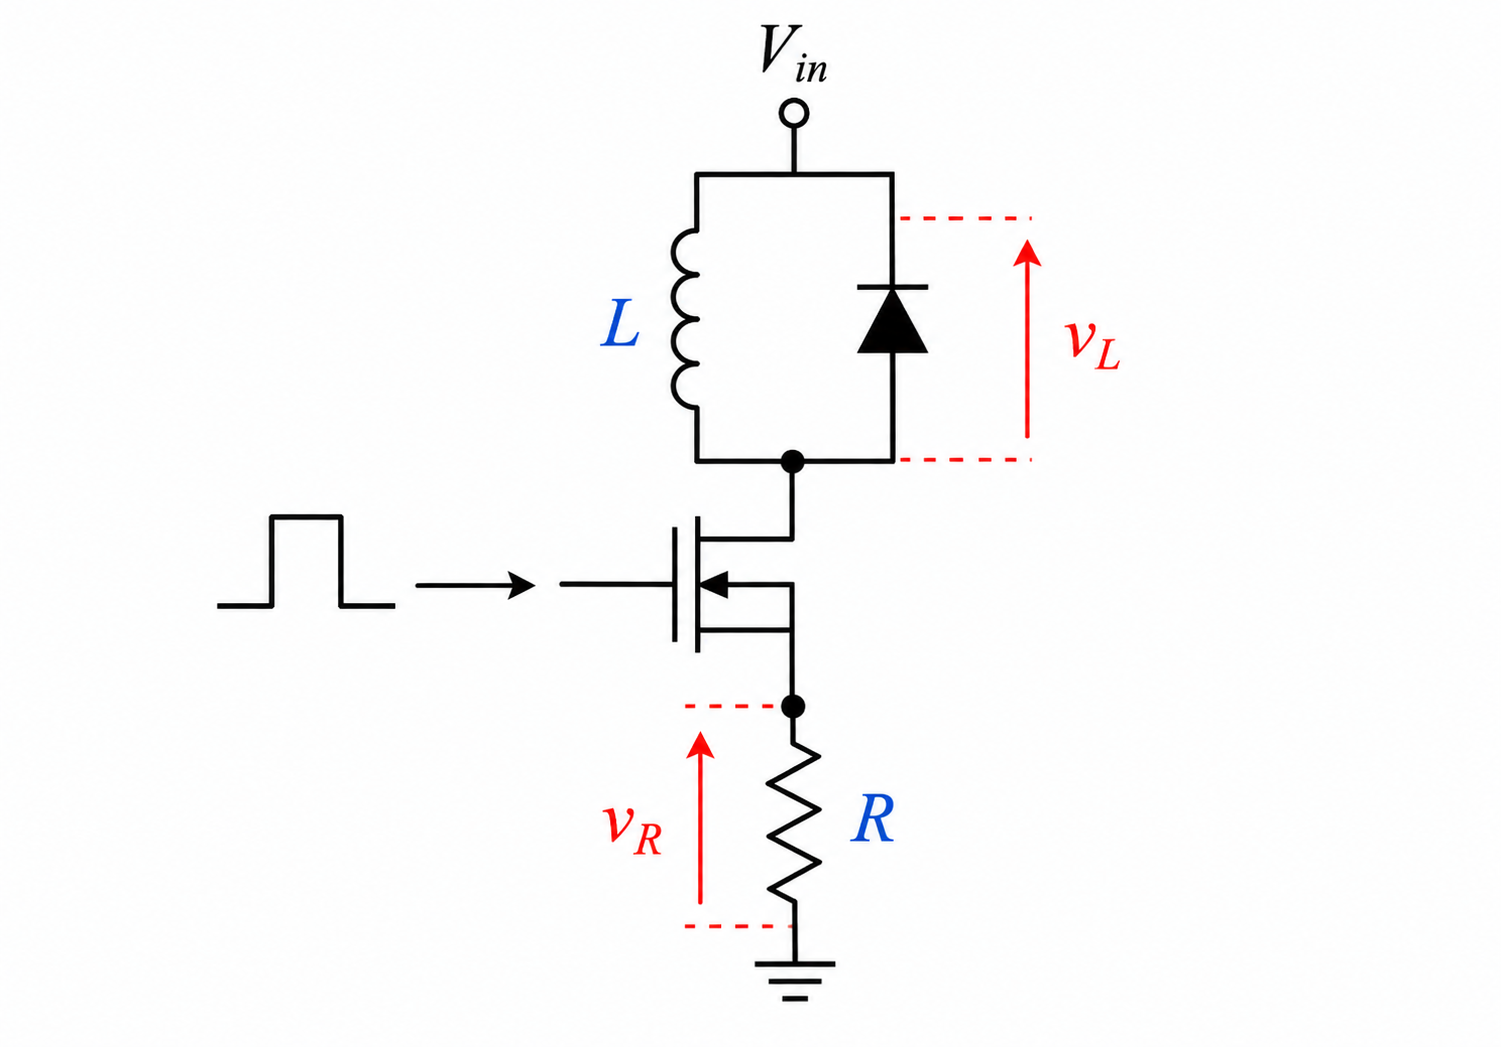
\includegraphics[width = 0.6\textwidth]{img/inductor/circuito_inductor.png}
\caption{Circuito utilizado para caracterizar el inductor.}
\label{fig:circuito_inductor}
\end{figure}

Dado que la resistencia de sensado es pequeña, su corriente ha de ser aproximadamente igual a la corriente que circula por el inductor. La misma, será proporcional a la tensión del resistor:
\[
\Delta i_L = R \, \Delta v_R\,.    
\]

Dado que $v_L = L \cdot \Delta i_L / \Delta t$ y $v_L = V_\text{in} - \Delta v_R$ se obtiene 
\[
L = \frac{V_\text{in} - \Delta v_R}{\Delta i_L / \Delta t} \, .
\]

En la Figura~\ref{fig:lineal} se observa la tensión del resistor, de donde se obtuvo vía cursores $\Delta t = 100\,\upmu$s y $\Delta v_R = 1.1\,$V, por lo que se obtiene una inductancia $L = 408.7\,\upmu$H, un valor superior al diseñado pero aún muy por encima de la inductancia mínima necesaria.

Asimismo, en la Figura~\ref{fig:saturacion} se observa que el inductor llego a la zona de saturación dado el punto de inflexión en la característica a una corriente de saturación $I_S = 4\,$A.

\begin{figure}[H]
\centering
\begin{subfigure}{0.48\textwidth}
\centering
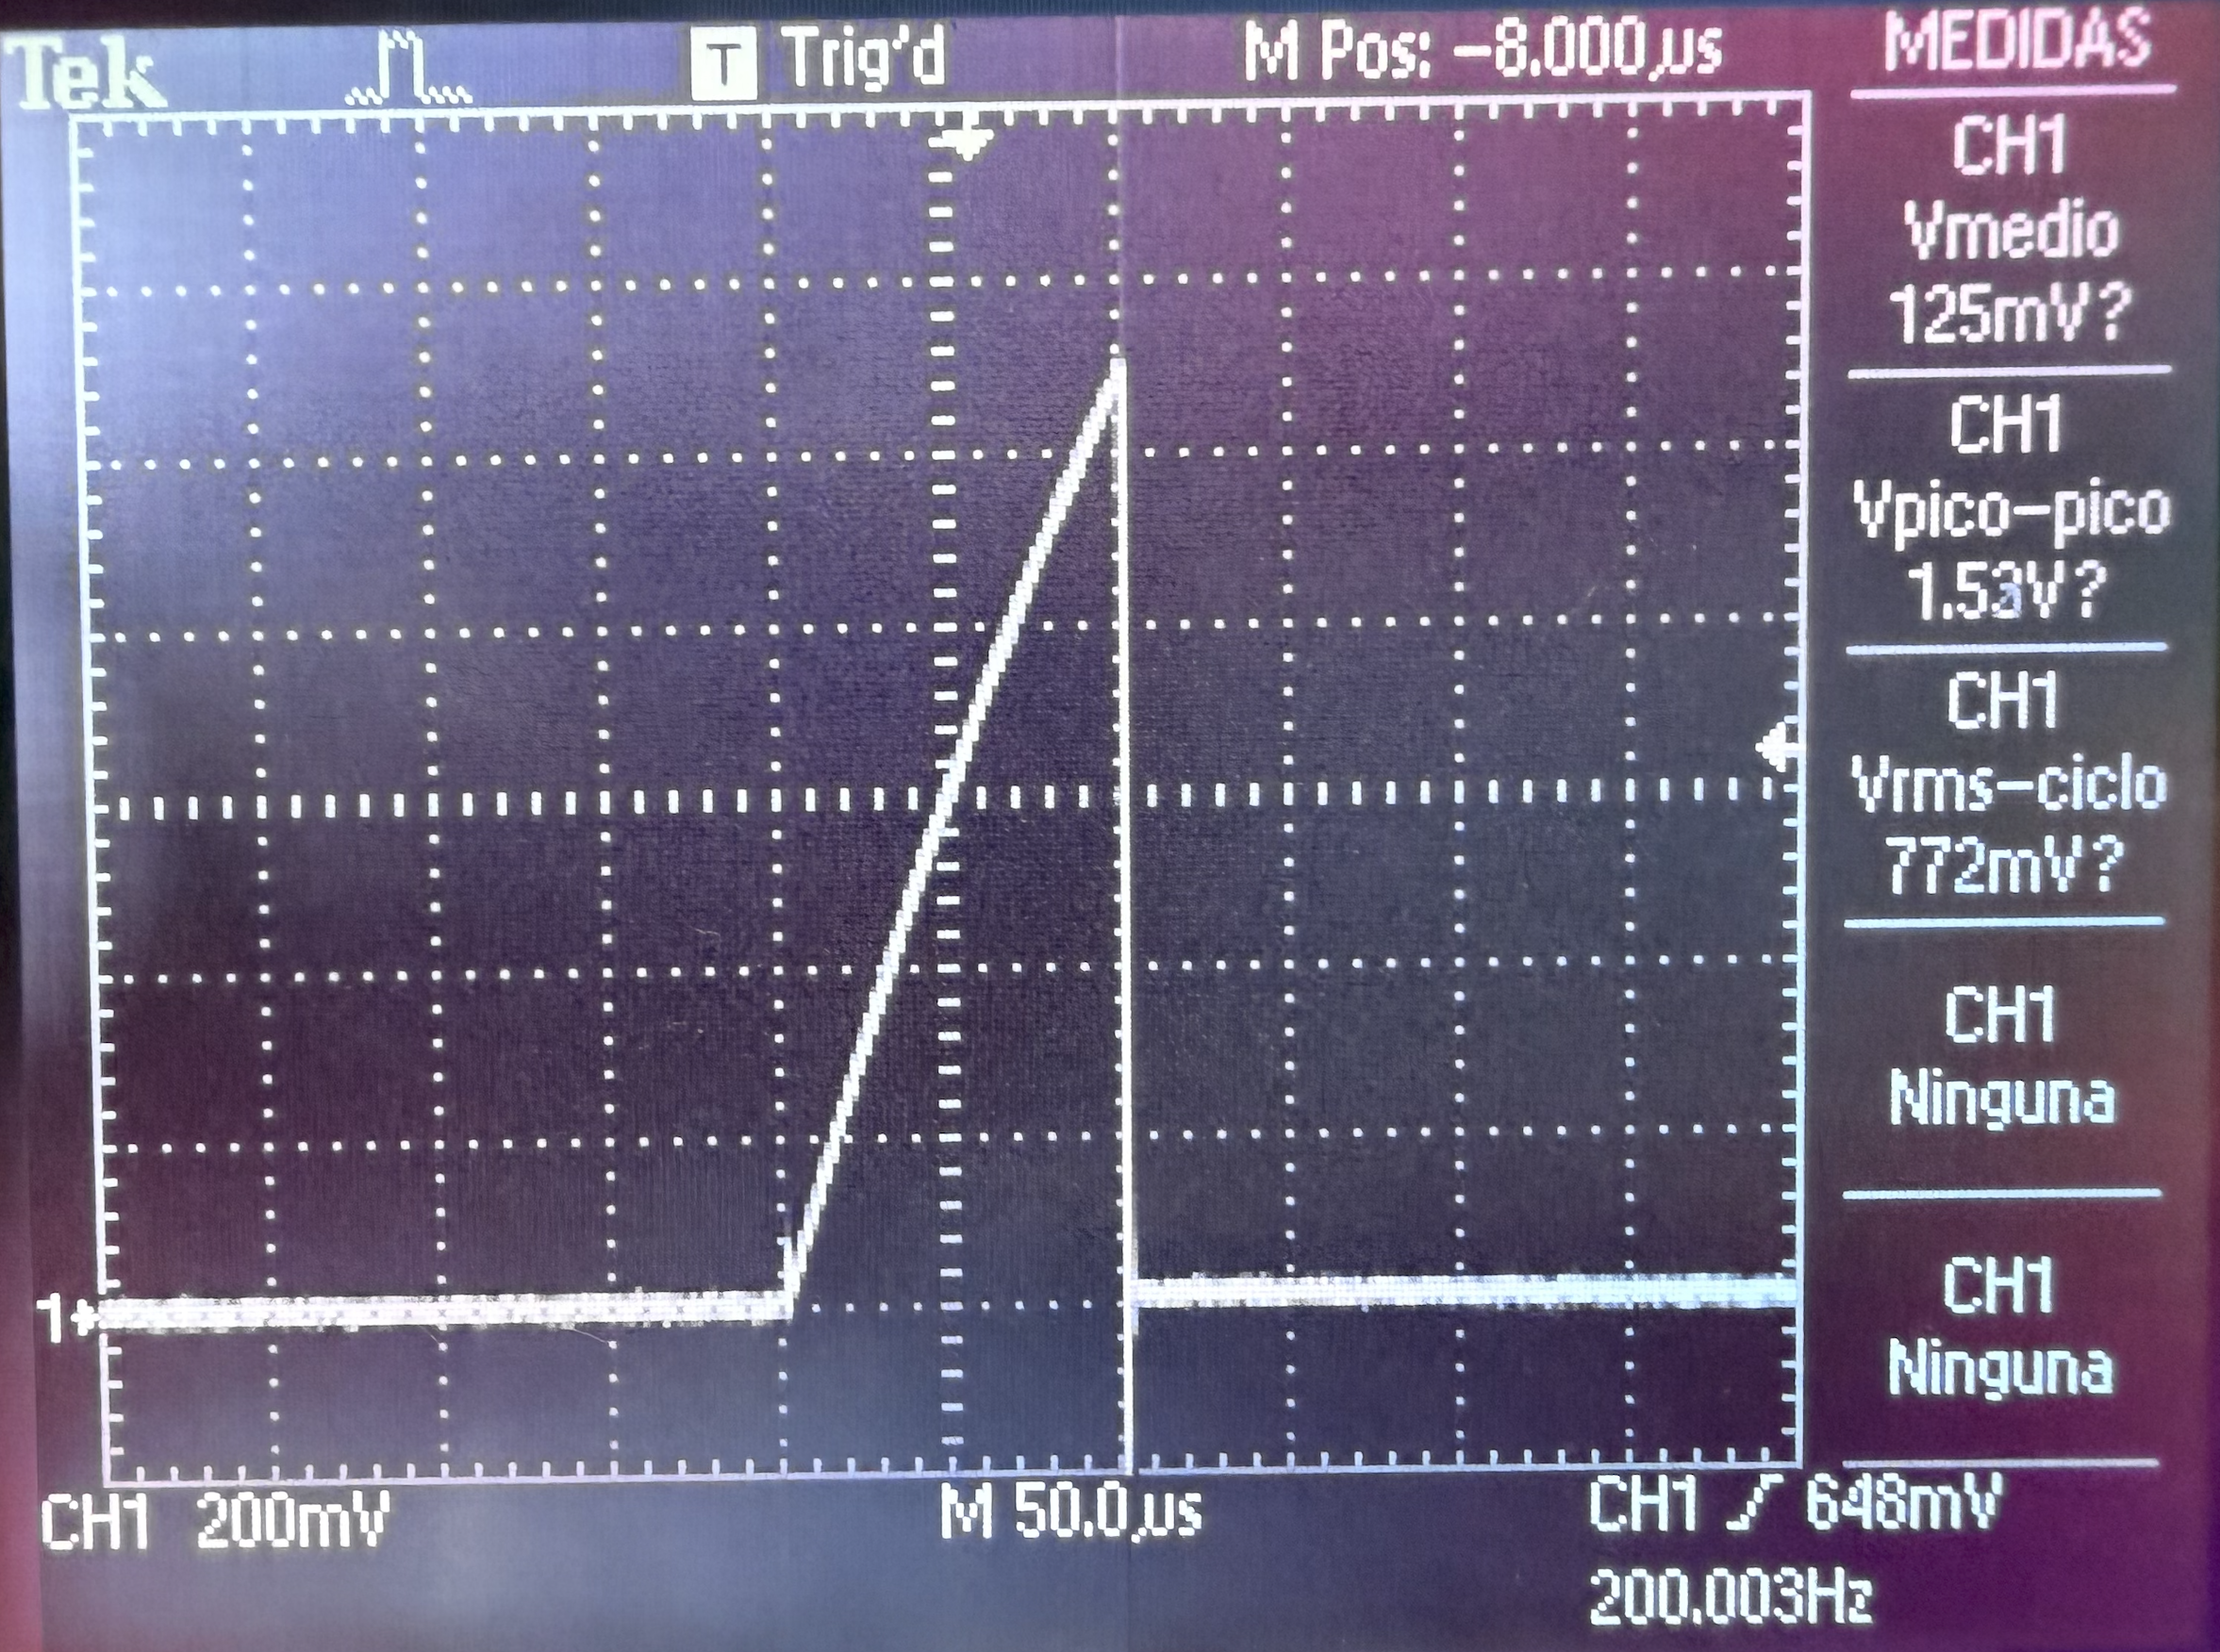
\includegraphics[width=\textwidth]{img/inductor/lineal.png}
\caption{Tensión en el resistor (zona lineal).}
\label{fig:lineal}
\end{subfigure}
\hfill
\begin{subfigure}{0.48\textwidth}
\centering
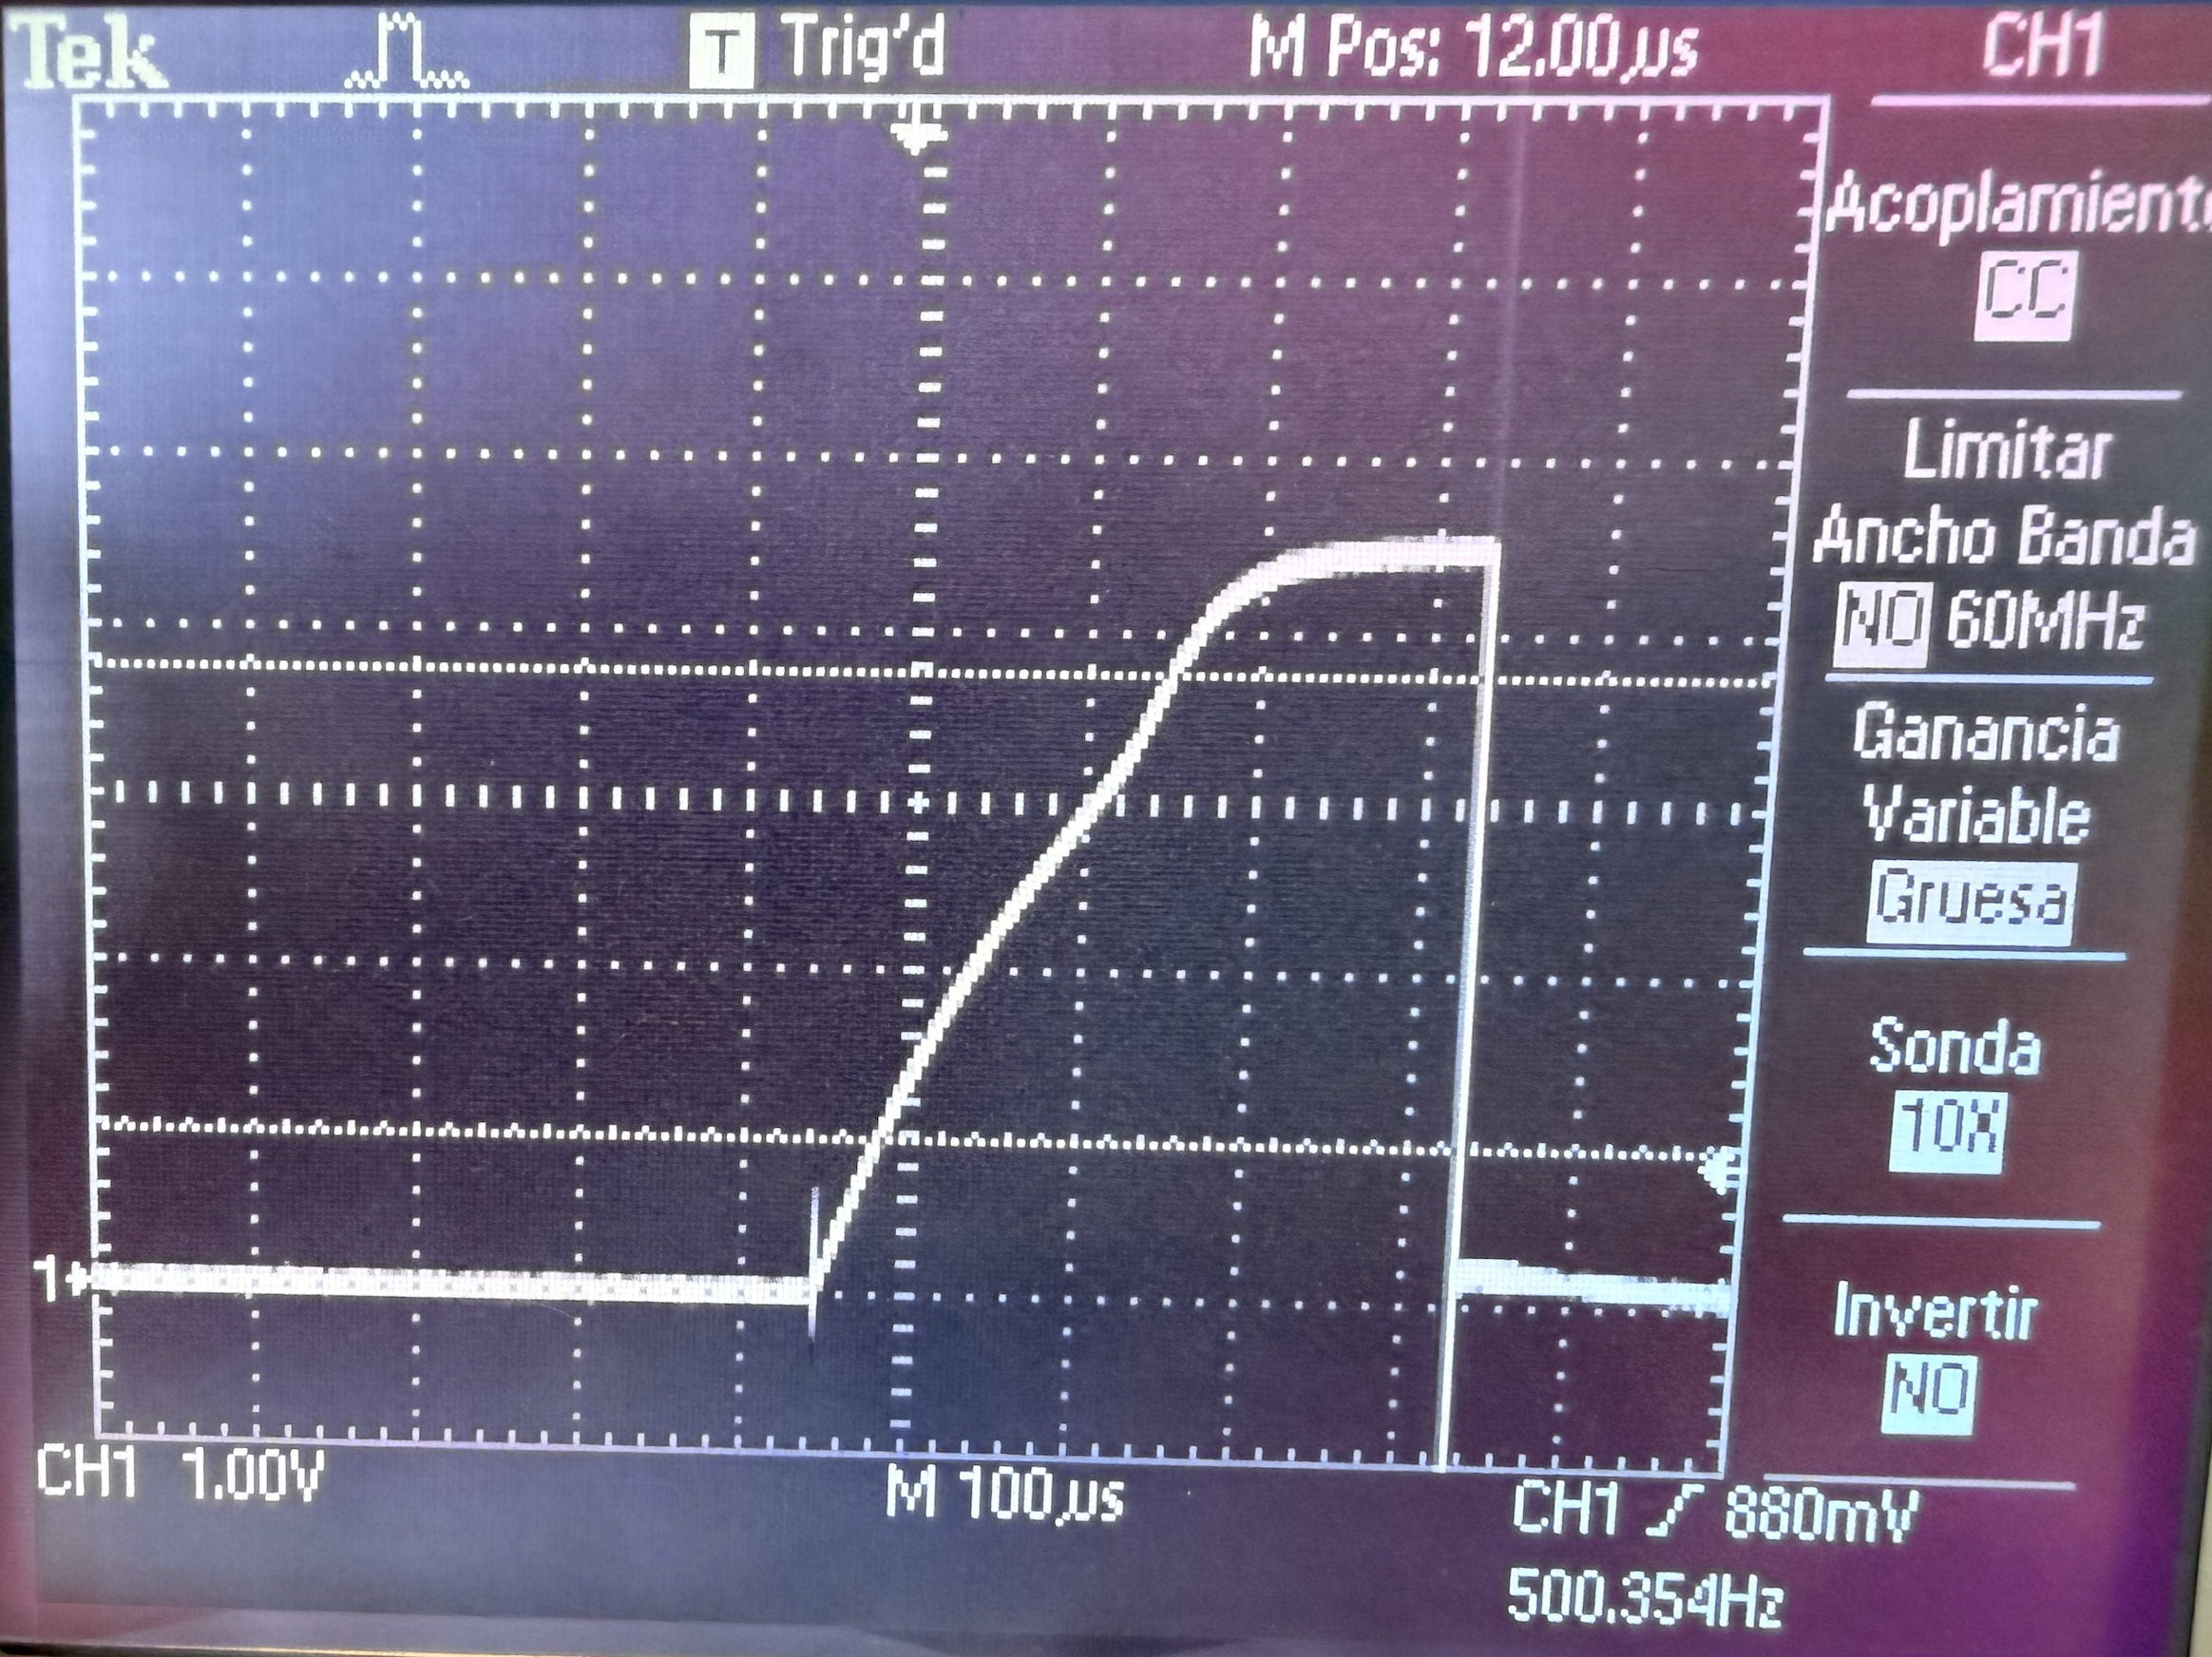
\includegraphics[width=\textwidth]{img/inductor/saturacion.png}
\caption{Tensión en el resistor (saturación).}
\label{fig:saturacion}
\end{subfigure}
\caption{Mediciones utilizadas para caracterizar el inductor.}
\label{fig:mediciones_inductor}
\end{figure}

La densidad de flujo magnético puede estimarse mediante
\[
B = \frac{A_L \, n \, I}{A_c}\,.
\]

Evaluando la expresión para la corriente de saturación se obtiene $B_{\max} = 0.439\ \text{T}\,$. Este resultado concuerda con la curva \(B\)-\(H\) del material CF196 mostrada en la Figura~\ref{fig:campo}, donde puede observarse que la región de saturación comienza aproximadamente para densidades de flujo comprendidas entre \(430\) y \(450\,\text{mT}\). En consecuencia, una corriente de \(4\,\text{A}\) sitúa al núcleo muy próximo al inicio de la saturación magnética, justificando su adopción como corriente máxima de operación.

\begin{figure}[H]
    \centering
    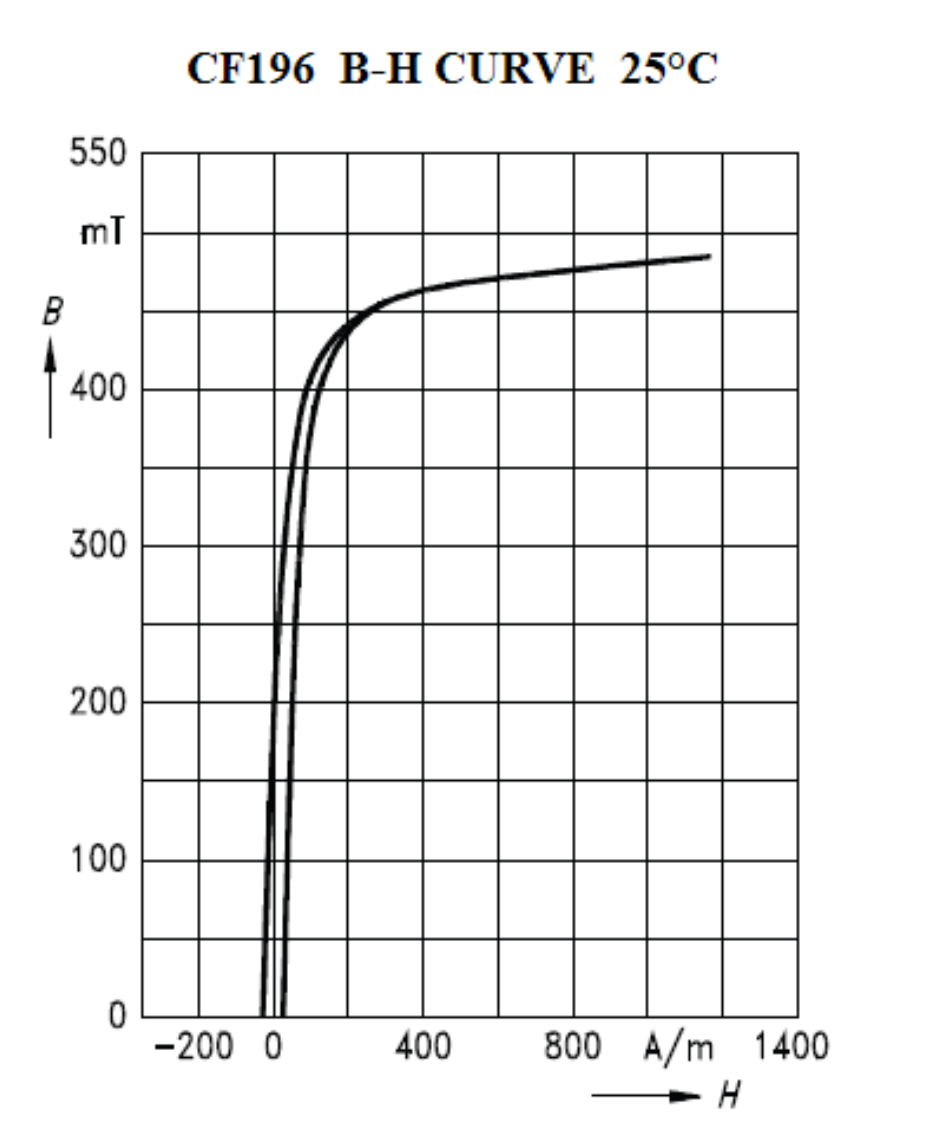
\includegraphics[width = 0.5\textwidth]{img/inductor/campo.png}
    \caption{Curva \(B\)-\(H\) del material CF196 a 25°.}
    \label{fig:campo}
\end{figure}